\chapter{An Efficient Algorithm for Type-Safe Structural Diffing}

\section{Abstract}
Effectively computing the difference between two versions of a source file has become an indispensable part of software development. The de facto standard tool used by most version control systems is the UNIX diff utility, that compares two files on a line-by-line basis without any regard for the structure of the data stored in these files. This paper presents an alternative datatype generic algorithm for computing the difference between two values of any algebraic datatype. This algorithm maximizes sharing between the source and target trees, while still running in linear time. Finally, this paper demonstrates that by instantiating this algorithm to the Lua abstract syntax tree and mining the commit history of repositories found on GitHub, the resulting patches can often be merged automatically, even when existing technology has failed.

\section{Introduction}
\begin{itemize}
    \item A consequence of the by line granularity of the UNIX diff is it inability to identify more fine-grained changes in the objects it compares.
    \item Ideally, however, the objects under comparison should dictate the granularity of change to be considered. This is precisely the goal of structural differencing tools.
    \item In this paper we present an efficient datatype-generic algorithm to compute the difference between two elements of any mutually recursive family
    \item The \textit{diff} function computes these differences between two values of type \textit{a}, 
    \item and \textit{apply} attempts to transform one value according to the information stored in the
    \textit{Patch} provided to it.
    \item We expect certain properties of our diff and apply functions.
    \begin{itemize}
        \item The first being \textit{correctness}: the patch that \textit{diff x y} computes can be used to faithfully reproduces \textit{y} from \textit{x}.
        \[
            \forall \: x \: y \: . \: apply (diff \: x \: y) \: x \: \equiv \: Just \: y
        \]
        \item The second being \textit{preciseness}:
        \[
            \forall \: x \: y \: . \: apply (diff \: x \: x) \: y \: \equiv \: Just \: y
        \]
        \item The last being \textit{computationally efficient}: Both the \textit{diff} and \textit{apply} functions needs to be space and time efficient.
    \end{itemize}
    \item There have been several attempts at generalizing UNIX diff results to handle arbitrary datatypes, but following the same recipe: enumerate all combinations of insertions, deletions and copies that transform the source into the destination and choose the 'best' one. We argue that this design has two weaknesses when generalized to work over arbitrary types:
    \begin{itemize}
        \item The non-deterministic nature of the design makes the algorithms inefficient.
        \item There exists no canonical 'best' patch and the choice is arbitrary.
    \end{itemize}
    \item This paper explores a novel direction for differencing algorithms: rather than restricting ourselves to \textit{insertions, deletions,} and \textit{copy operations}, we allow the \textit{arbitrary reordering, duplication,} and \textit{contraction of subtrees}.
\end{itemize}

\section{Tree Diffing: A Concrete Example}
\begin{itemize}
    \item We explicitly model permutations, duplications and contractions of subtrees within our notion of \textit{change}. Where contraction here denotes the partial inverse of a duplication.
    \item The representation of a \textit{change} between two values of type \inlinehaskell{Tree23}, is given by identifying the bits and pieces that must be copied from source to destination making use of permutations and duplications where necessary.
    \item A new datatype \inlinehaskell{Tree23C} $\varphi$, enables us to annotate a value of \inlinehaskell{Tree23} with holes of $\varphi$. Therefore, \inlinehaskell{Tree23C MetaVar} represents the type of \inlinehaskell{Tree23} with holes carrying metavariables.
    \item These metavariables correspond to arbitrary trees that are \textit{common subtrees} of both the source and destination of change.
    \item We refer to a value of \inlinehaskell{Tree23C} as a \textit{context}.
    \item A \textit{change} in this setting is a pair of such contexts. The first context defines a pattern that binds some metavariables, called the \textbf{deletion context}; the second, called the \textbf{insertion context}, corresponds to the tree annotated with the metavariables that are supposed to be instantiated by the binding given by the deletion context.
    \begin{haskell}
        type Change23 !$\varphi$! = (Tree23C !$\varphi$!, Tree23C !$\varphi$!)
    \end{haskell}
    \item Applying a change is done by instantiating the metavariables in the deletion context and the insertion context:
    \begin{haskell}
        applyChange :: Change23 MetaVar -> Tree23 -> Maybe Tree23
        applyChange (d, i) x = del x >>= ins i
    \end{haskell}
    \item The changeTree23 function merely has to compute the deletion and insertion contexts
    \begin{haskell}
        changeTree23 :: Tree23 -> Tree23 -> Change23 MetaVar
        changeTree23 s d = (extract (wcs s d) s, extract (wcs s d) d)
    \end{haskell}
    \item The extract function receives an oracle and a tree. It traverses its argument tree, looking for opportunities to copy subtrees.
    \begin{haskell}
        extract :: (Tree23 -> Maybe MetaVar) -> Tree23 -> Tree23C MetaVar
        extract o t = maybe (peel t) Hole (o t)
            where peel Leaf = LeafC
                  peel (Node2 a b)   
                    = Node2C (extract o a) (extract o b)
                  peel (Node3 a b c) 
                    = Node3C (extract o a) (extract o b) (extract o c)
    \end{haskell}
    \item This iteration of the changeTree23 function has a subtle bug: not all common subtrees can be copied. In particular, we cannot copy a tree t that occurs as a subtree of the source and destination, but also appears as a subtree of another, larger common subtree.
    \item One way to solve this is to introduce an additional post-processing step that substitutes the variables that occur exclusively in the deletion or insertion context by their corresponding tree.
    \begin{haskell}
        changeTree23 :: Tree23 -> Tree23 -> Change23 MetaVar
        changeTree23 s d 
            = postprocess s d (extract (wcs s d) s) (extract (wcs s d) d)
    \end{haskell}
\end{itemize}

\subsection{Minimizing Changes}
\begin{itemize}
    \item The process of minimizing and isolating the changes starts by identifying the redundant part of the contexts. That is, the constructors that show up as a prefix in both the deletion and the insertion context.
    \item They are essentially being copied over, and we want to make this fact explicit by separating them into what we call the \textit{spine} of the patch.
    \item If a constructor is in the spine, we know it has been copied, if it shows up in a change, we know it was either deleted or inserted.
    \begin{haskell}
        type Patch23 = Tree23C (Change23 MetaVar)

        patch :: Patch23
        patch = Node3C (Hole (Hole 0, Hole 0))
                       (Hole (Node2C (Hole 0) (Hole 1)
                             , Node2C (Hole 1) (Hole 0)))
                       (Node2C (Hole (tree23ToC w, tree23ToC w'))
                               (Hole (Hole 3, Hole 3)))
    \end{haskell}
    \begin{figure}[H]
        \centering
        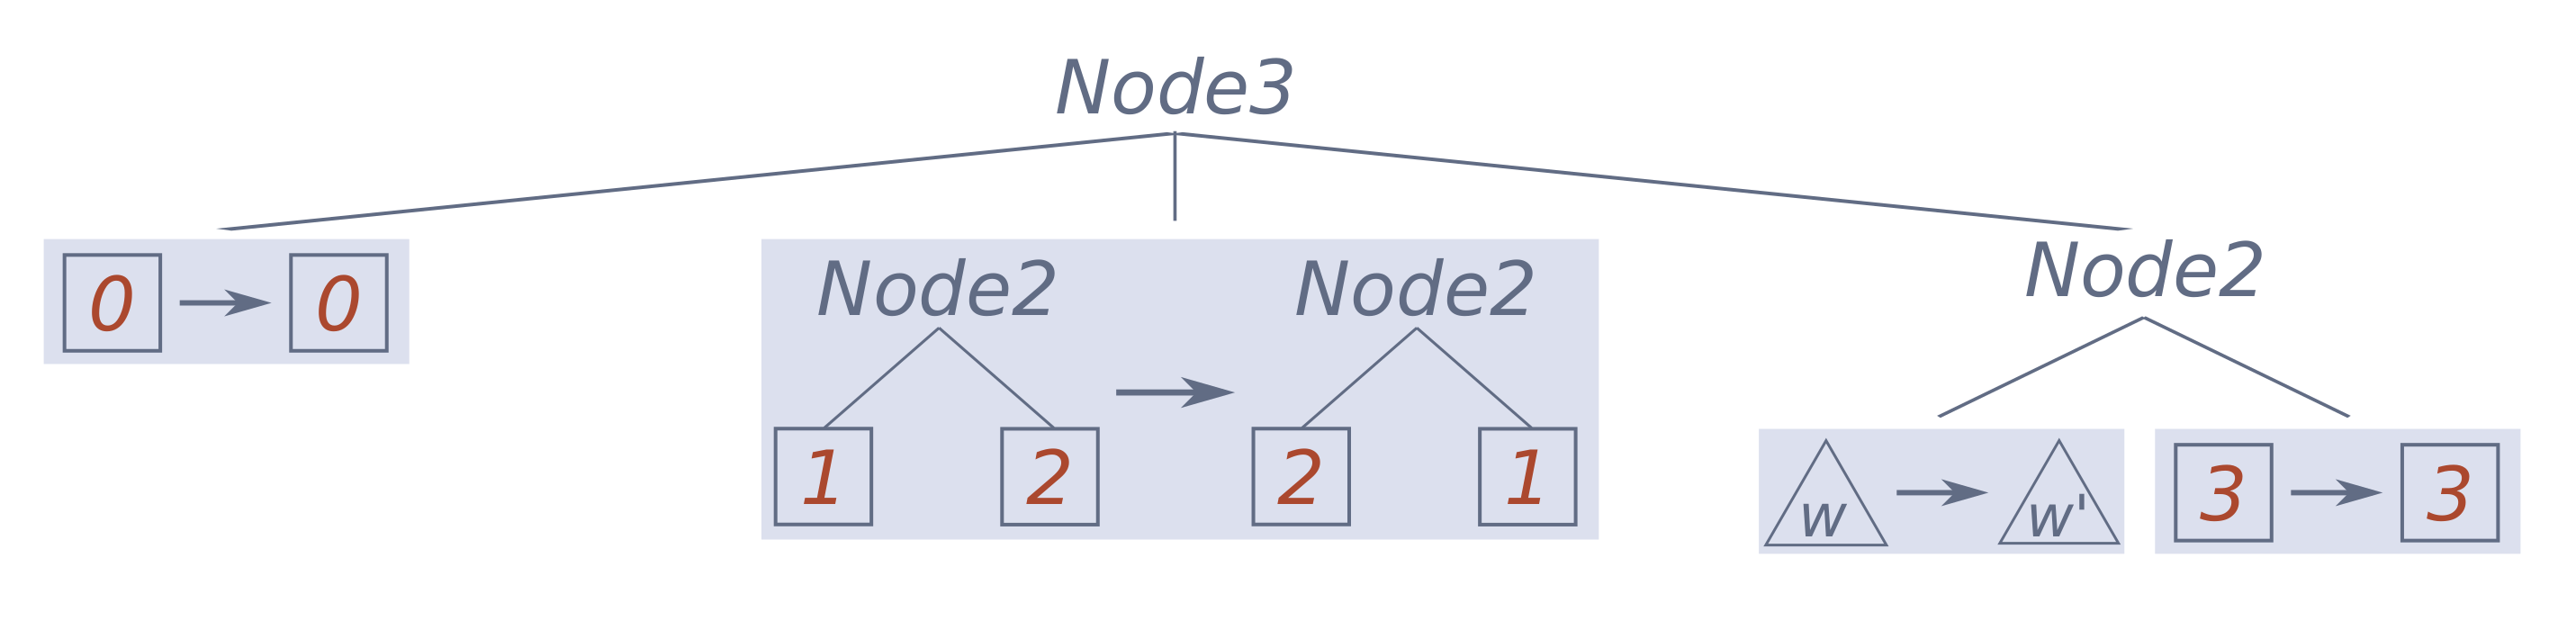
\includegraphics[width=.8\textwidth]{summaries/patch_tree23.png}
        \caption{Patch23 Example}
        \label{fig:patch_tree23}
    \end{figure}
    \item A patch consists in a spine with changes inside it. Figure \ref{fig:patch_tree23} illustrates a value of type Patch23, where the changes are visualized with a shaded background in the leaves of the spine.
    \item The first step to compute a patch from a change is identifying its spine.
    \item We are essentially splitting
    a monolithic change into the greatest common prefix of the insertion and deletion contexts, leaving smaller changes on the leaves of this prefix:
    \begin{haskell}
        gcp :: Tree23C var -> Tree23C var -> Tree23C (Change23 var)
        gcp LeafC LeafC = LeafC
        gcp (Node2C a1 b1) (Node2C a2 b2) 
            = Node2C (gcp a1 a2) (gcp b1 b2)
        gcp (Node3C a1 b1 c1) (Node3C a2 b2 c2)
            = Node3C (gcp a1 a2) (gcp b1 b2) (gcp c1 c2)
    \end{haskell}
    \item The greatest common prefix consumes all the possible constructors leading to disagreeing parts of the contexts where this might be too greedy.
    \item To address this problem, we go over the result from our call to \inlinehaskell{gcp}, pulling changes up the tree until each change is closed, that is, the set of variables in both contexts is identical. We call this process the closure of a patch
    \item The final diff function for \inlinehaskell{Tree23} is then defined as follows:
    \begin{haskell}
        diffTree23 :: Tree23 -> Tree23 -> Patch23
        diffTree23 s d = closure $ gcp $ changeTree23 s d
    \end{haskell}
\end{itemize}

\subsection{Defining the \inlinehaskell{wcs} for \inlinehaskell{Tree23}}

\begin{itemize}
    \item In order to have a working version of our diff algorithm for Tree23 we must provide the wcs implementation. Recall that the wcs function, \textit{which common subtree}, has type:
    \begin{haskell}
        wcs :: Tree23 -> Tree23 -> Tree23 -> Maybe MetaVar
    \end{haskell}
    \item Given a fixed \textit{s} and \textit{d}, \textit{wcs s d x} returns Just \textit{i} if \textit{x} is the $i^{th}$ subtree of
    \textit{s} and \textit{d} and Nothing if \textit{x} does not appear in \textit{s} or \textit{d}.
    \item To tackle the first issue and efficiently compare trees for equality we will be using cryptographic hash functions to construct a fixed length bitstring that uniquely identifies a tree modulo hash collisions.
    \item Said identifier will be the hash of the root of the tree, which will depend on the hash of every subtree, much like a Merkle tree
    \begin{haskell}
        merkleRoot :: Tree23 -> Digest
        merkleRoot Leaf = emptyDigest
        merkleRoot (Node2 x y)
            = hash (concat ["node2", merkleRoot x, merkleRoot y])
        merkleRoot (Node3 x y z)
            = hash (concat ["node3", merkleRoot x, merkleRoot y, merkleRoot z])
    \end{haskell}
    \item the ($\equiv$) definition above is still
    linear, we recompute the hash on every comparison. We fix this by caching the hash associated with every node of a Tree23. This is done by the decorate function
    \begin{haskell}
        data Tree23H = LeafH
                     | Node2H (Tree23H, Digest) (Tree23H, Digest)
                     | Node3H (Tree23H, Digest) 
                              (Tree23H, Digest) 
                              (Tree23H, Digest)
    \end{haskell}
    \item This enables us to define a constant time merkleRoot function, shown below, which makes the ($\equiv$) function run in constant time.
    \begin{haskell}
        merkleRoot :: Tree23H -> Digest
        merkleRoot LeafH = emptyDigest
        merkleRoot (Node2H (_, hx) (_, hy)) 
            = hash (encode "2" ++ hx ++ hy)
        merkleRoot (Node3H (_, hx) (_, hy) (_, hz))
            = hash (encode "3" ++ hx ++ hy ++ hz)
    \end{haskell}
\end{itemize}